\section{Results}
\label{sec:results}
In this section, we will first describe our data-collection process. Next we will show the code repair, 
and detection accuracy techniques on a small subset of this collected dataset.   

\subsection{Data collection} 
  For experimental evaluation, We turn to the datasets from two previous sources ~\cite{meng2018secure,fischer2017stack}. 
  Both of these dataset contain code snippets posted on Stack Overflow. 
  Fisher et al. crawled 1,161 code snippets posted on Stack Overflow related to Andrioid security ~\cite{fischer2017stack}. 
  They considered a code snippet related to Android security if the code snippets makes API calls to
  one of the security services such as Java cryptography, Java secure communications, public key infrastructure X.509 certificates, 
  and Java authentication - authorization services. The popular crypto libraries used by Andriod developers such as Bouncy Castle, 
  SpongyCastle, Apache TLS/SSL, keyczar, jasypt, and GNU Crypto were also included. 
  
  Meng et al.  extracted 503 code snippets from 22,195 Stack Overflow posts by filtering the posts based on votes, duplications, 
  and absence of code snipeets~\cite{meng2018secure}. In total the dataset used in this experiments,  is generated by combining these two. 
  Our dataset contains 1,664 code snippets. The timeline of these code snippets are from 2008-2017.
  %\minote{add some more info and some statistics}
 % Since it would very time consuming to manually analysis 1.6K code snippets to get the ground truth, 
  %we randomly sample  half of the code snippets from the available corpus which is 800. 
  Upon manual inspection we filter out 363 as they were not related to security, and carry the experimental evaluation on 1273 code snippets 
  For the rest of the experiments we will only consider these 1301 code snippets.
    The average size of these %800 
  code snippets is 46 LoC having a very high standard deviation of 58. 


%\subsection{Data processing and categorization}
%  We manually analysis 
%  As to get the ground truth of the presence of insecure pattern, we have to manully analysis them, it becomes very time consuming. Therefore to make the analysis less consuming time , we only consider randomly sampled 800 code snippets -- about half of the 1.6K code snippets available. 
%  We then assign the code snippets into one of the 8 insecure patterns.  %and record the common keywords appear in the code snippets. By doing this we have list of common keyword for each of the 8 insecure patterns. We can then categorize all 1.6K code snippets using these common keywords.
  

\subsection{Code repair success rate.} 
%AES: 85/225 Broken-Hash: 69/219 
% Constructor class
\begin{figure}[ht]
  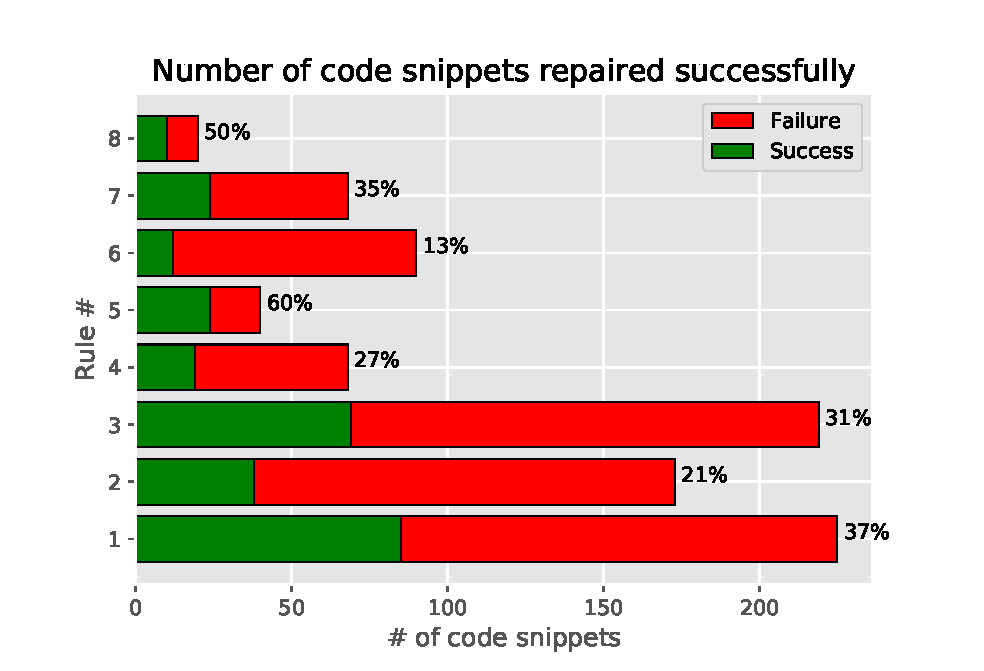
\includegraphics[width=\linewidth]{Figures/success_full_repair2.eps.eps}
  \caption{Percentage of code snippets successfully repaired. For each insecure pattern, we show the number 
  of code snippets we are able to convert to Jimple IR before and after applying code repairing.}
  \label{fig:code-repair}
\end{figure}

We call a code snippet successfully repaired if after applying the code repair techniques, we can convert it to a Jimple IR. 
We are able to convert 714 code snippets out of 1273 code snippets we have considered-- out which 401 of them was throwing exceptions
while converting them Jimple IR without any code repairs.  
Figure~\ref{fig:code-repair} 
illustrates the percentage of code snippets for each categorize, we have been able to parsed (i.e., convert to Jimple IR) before and after
the code repair techniques discussed in section~\ref{subsec:code-repair}.
In summary , we are able to parse 33\% more code snippets by code repairing.

%a repair accurarcy of 30.31\%. 
%We also categorize each converted into one more or category based on the secure/insecure use of the patterns presented on Table~\ref{tab:insecure-patterns}.  



\subsection{Insecure pattern detection accuracy.}
After converting each successfully repaired code snippets to Jimple IR, we detect insecure pattern 7, and 8 using keyword searching as mentioned previously. 
However for insecure pattern 1-6, need to apply backward flow analysis. To do this we give the Jimple IR to our tool. 
Out tool is built on top of CryptoGuard. 
CryptoGuard uses Soot as its program analysis engine. 
Using Soot's \texttt{JimpleAST} API~\footnote{\url{https://www.sable.mcgill.ca/soot/doc/soot/jimple/parser/JimpleAST.html}}, 
we can run backward flow analysis given the slicing criteria from Table~\ref{tab:slicing}. 
The idea is track the special method invocations parameter from the slicing criteria. 
In this way we can inspect the set of program statements which are affected 
by this slicing criteria, and figure out the presence of insecure patterns.



Table~\ref{tab:results} shows the total number of code snippets for of the 8 insecure patterns. 
%(they sum up to more than 813 as some code snippets has two or more rules). 
Parsed column refers to the number of code snippets, we have been able to convert to Jimple IR after applying the code repair discussed 
in section~\ref{subsec:code-repair}. We also shows the TP, FN, FN along side the precision, and recall rate.
As it can seen we have not been able to run backward flow analysis for insecure pattern 3. 
The reasons are explain the in the appendix~\ref{appendix:X509TrustManager}.
%If any of these set of program statements contains i) 
% Say you have done the  1,2,4,5, 7,8 correctely. How to present the results? 
% say you haven trying to address the problem of empty method detection but have not been able to do so. 

% Precision = tp/ (tp + fp)
% Recall = tp/ (tp + fn)

\begin{table}[ht]
\begin{tabular}{|c|r|r|r|r|r|r|r|}
\toprule
Insecure  Pattern \# & Parsed & TP & FP & FN & Precision & Recall \\ \midrule
1 & 225 & 186 & 39 & 0 & 100 & 82 \\
2 & 173 & 165 & 0 & 8 & 95 & 100 \\
\textcolor{red}{3} & \textcolor{red}{219} & \textcolor{red}{-} & \textcolor{red}{-} & \textcolor{red}{-} & \textcolor{red}{-} & \textcolor{red}{-}\\
4 & 68 & 61 &  0 & 8& 88 & 100 \\
5 & 40 & 37 & 0 & 3& 93 & 100 \\
6 & 90 & 81 & 7 & 2 & 91 & 91 \\ \midrule
7 & 68 & 63 & 0& 5 & 79 & 100 \\
8 & 20 & 11 & 0& 9 & 55 & 100\\ %\midrule 
%Total & 20 & 11 & 3& 0 & - & -\\        
\bottomrule
\end{tabular}
\caption{Precision and Recall of our analysis. Insecure pattern \#[7-8] where detected using keyword
searching. Insecure pattern \#[1-6] is detected using backward flow analysis. We are unable to detect
insecure pattern \#3 which is explained in appendix~\ref{appendix:X509TrustManager} 
}
\label{tab:results}
\end{table}


As we choose conservative keywords to  detect insecure pattern \#[7-8], 
both of them fails to detect cases some cases where insecure patterns occurs i.e., low precision. 
For backward flow analysis based detection inseucre patterns \#[1-6] has high accuracy and recall rate.